\documentclass[a4paper,oneside, 10pt]{article}
\usepackage[margin=0.7in]{geometry}
\usepackage[utf8]{inputenc}

\usepackage[cm-default]{fontspec}
\usepackage{xunicode, amsmath}
\usepackage{xltxtra}
\usepackage{pmboxdraw}

\usepackage{xgreek}
\usepackage{listings}
\lstset{basicstyle=\footnotesize\ttfamily,breaklines=true}

\setmainfont[Mapping=tex-text]{CMU Serif}

\usepackage{graphicx}

\makeatletter
\def\maxwidth{%
  \ifdim\Gin@nat@width>\linewidth
    \linewidth
  \else
    \Gin@nat@width
  \fi
}
\makeatother


\title{\textbf{Σχεδίαση Συστημάτων Αυτομάτου Ελέγχου} \\ 1η Άσκηση \\ \large{Σχεδίαση Ελεγκτών PID στο MATLAB / Simulink} \\ \small 6o Εξάμηνο - Ακ. Έτος 2017-18 - Ροή Σ}
\author{Μάριος Παπαχρήστου (03115101 - \texttt{papachristoumarios@gmail.com}) }
\date{\hrule}

\begin{document}

\maketitle

\section*{1o Ερώτημα} 

Δίνεται το σύστημα (plant) με συνάρτηση μεταφοράς $$G_p (s) = \frac {4500K} {s(s + 361.2)}$$ το οποίο θα ελέγξουμε με PD ελεγκτή $$G_c(s) = k_p + k_d s = $$ με προδιαγραφές για είσοδο $r(t) = t $ : $e_{ss} \le 0.000443, \; M_p \le 5 \%, \; T_r \le 0.005 \mathrm s, \; T_s \le 0.005 \mathrm s$

Το σύστημα έχει συνάρτηση μεταφοράς ανοικτού βρόχου την $$G(s) = G_c(s) G_p(s) = 
\frac { 4500K (k_p + k_d s) }  {s (s + 361.2) } $$ και συνάρτηση κλειστού βρόχου την 
$$\frac {Y(s)} {R(s)} = \frac {G(s)} {1 + G(s)} = \frac {4500 K k_p +  4500 K k_ds} {s^2 + (361.2 + 4500Kk_d)s + 4500 K k_p  }$$


Χωρίς τον ελεγκτή ο ΓΤΡ του ΣΚΒ του $G_p(s)$ είναι 

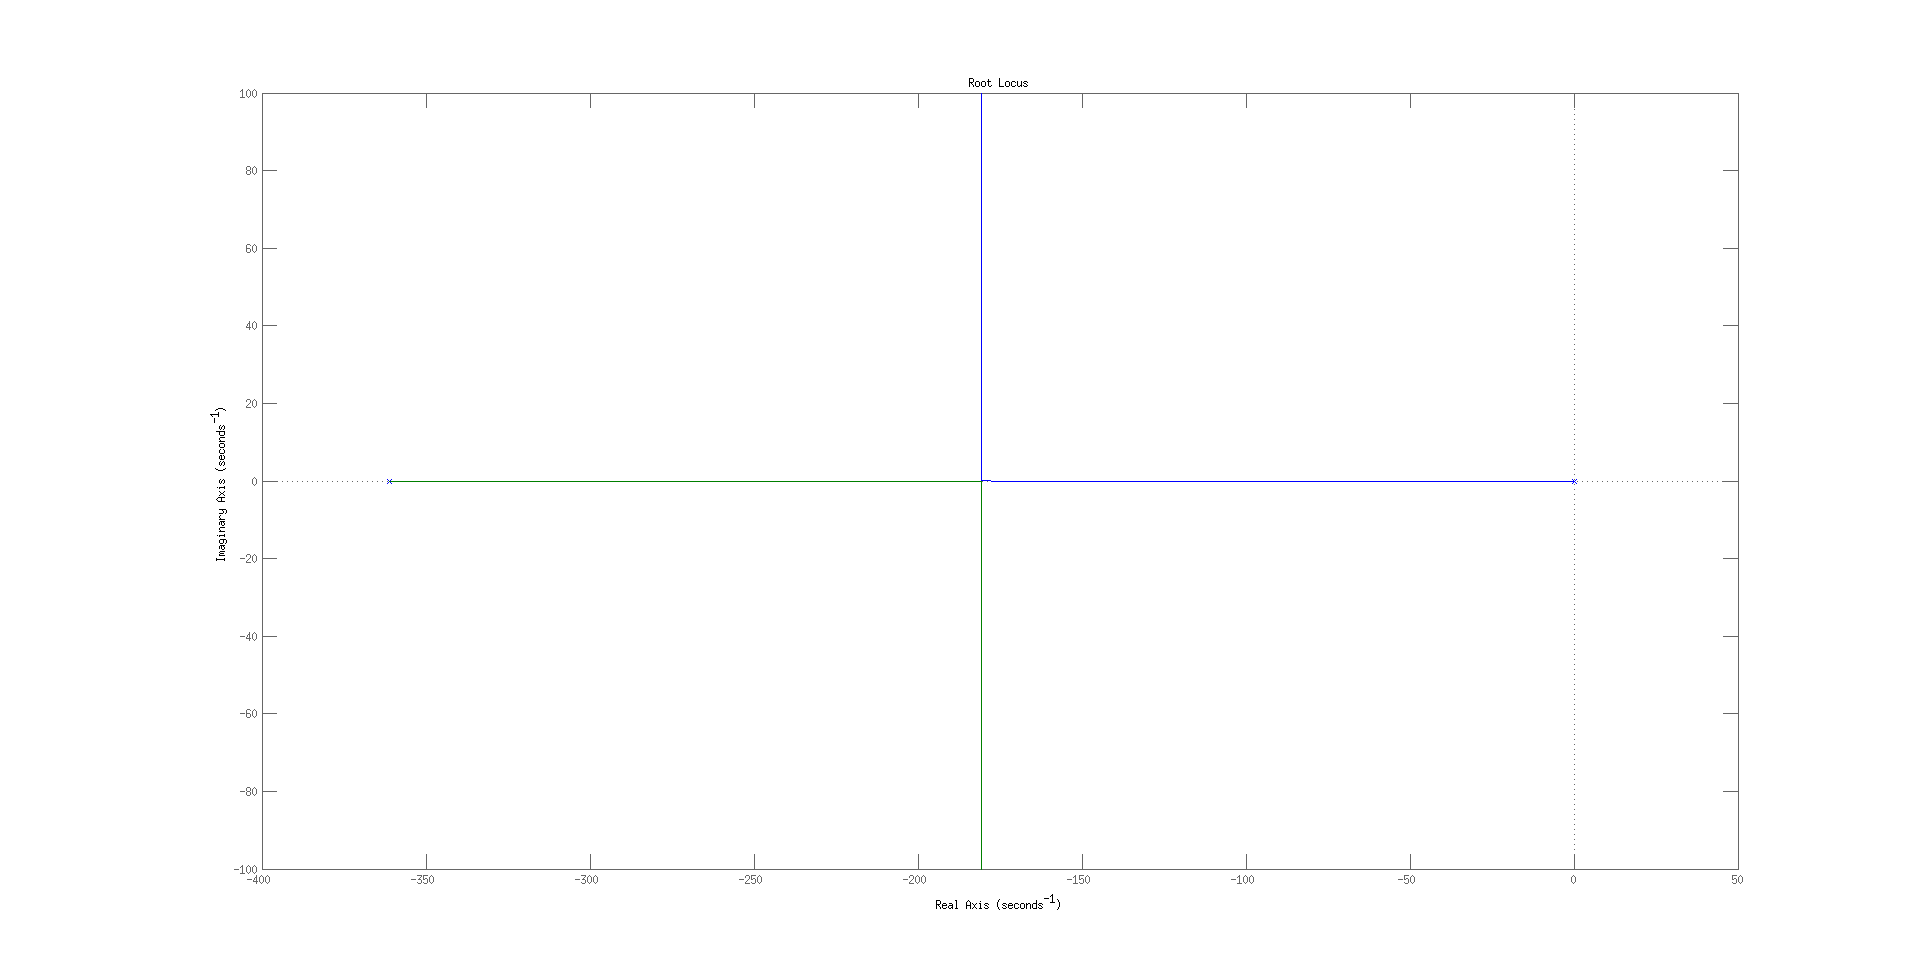
\includegraphics[width=\textwidth]{plant_rlocus.png}
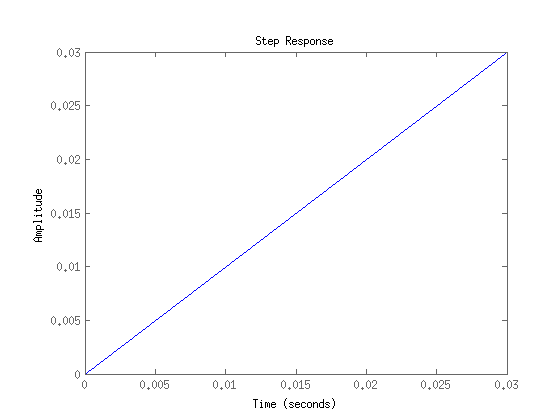
\includegraphics[width=\textwidth]{step1.png}


\subsection*{Περιορισμοί Σχεδίασης \& Σχεδίαση PD Controller} 


\paragraph{Σφάλμα στη μόνιμη κατάσταση} Αρχικά θέλουμε το σφάλμα μόνιμης κατάστασης να πληροί τον περιορισμό $e_{ss} \le 0.000443$. Το σφάλμα μόνιμης κατάστασης για είσοδο ράμπα δίνεται ως $$e_{ss} = \frac 1 {K_v}  \quad \mathrm{όπου} \quad K_v = \lim_{s \to 0} sG(s) = \frac {4500Kk_p} {361.2}$$ 

\paragraph{Επιλογή κερδών PD Controller} 
Μπορούμε να λάβουμε με διαδοχικές δοκιμές σε υποψήφια διαστήματα τιμές για τα κέρδη του PD που ικανοποιούν τους σχεδιαστικούς περιορισμούς για τα $T_r, T_s, M_p, e_{ss}$ τα οποία ελέγχουμε με τη συνάρτηση \texttt{stepinfo} στο MATLAB. Τέτοιες δοκιμές μας έδωσαν για $k_p = 1000, \; k_d = 3$ τα εξής αποτελέσματα
\begin{verbatim}
ess =

   8.0267e-05

>> params

params = 

        RiseTime: 1.6377e-04
    SettlingTime: 2.9665e-04
     SettlingMin: 0.9027
     SettlingMax: 0.9983
       Overshoot: 0
      Undershoot: 0
            Peak: 0.9983
        PeakTime: 7.7952e-04

\end{verbatim}  

τα οποία ικανοποιούν τους σχεδιαστικούς περιορισμούς μας. Επομένως ο PD ελεγκτής είναι ο $$G_c(s) = 1000 + 3s = 3 (s + 1000 / 3)$$

Ο γτρ του νέου συστήματος ανοικτού βρόχου $G(s)$ είναι

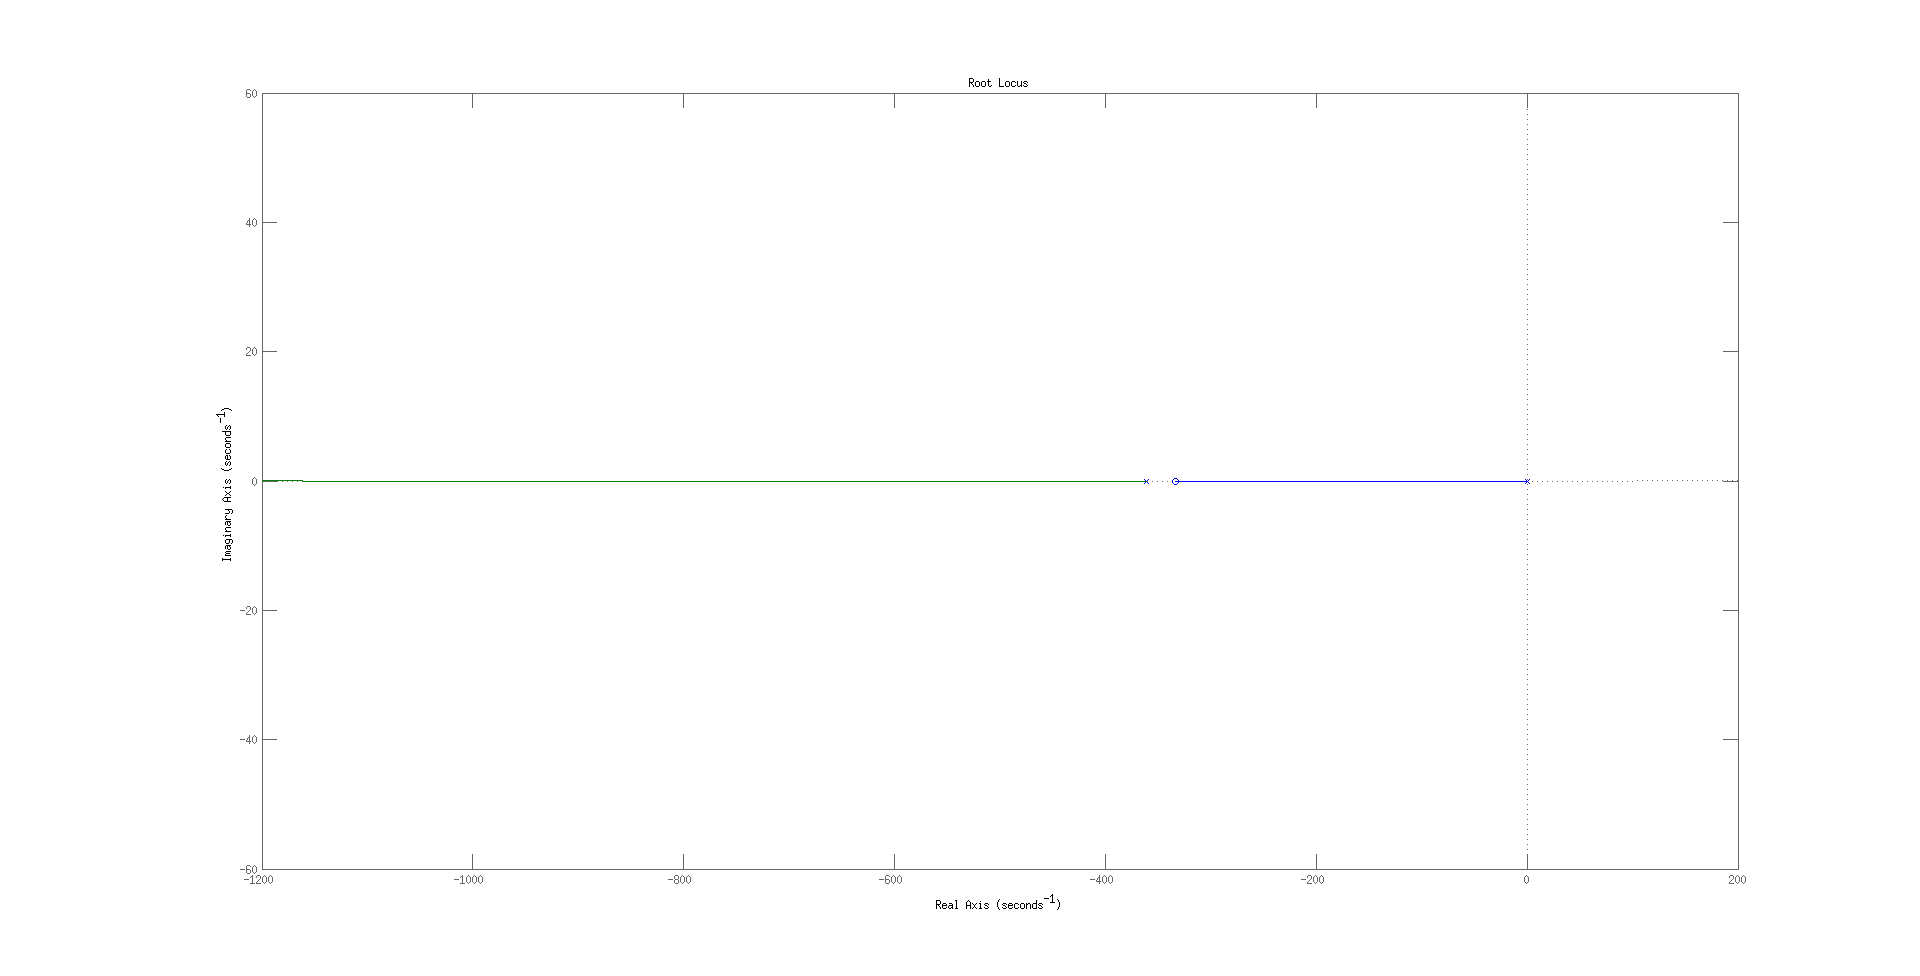
\includegraphics[width=\textwidth]{pd_rlocus.png}
 
\section*{2o Ερώτημα} 

Στο παρόν ερώτημα θα χρησιμοποιήσουμε PI ελεγκτή με συνάρτηση μεταφοράς $$G_c(s) = k_p + \frac {k_i} s$$ με σχεδιαστικούς περιορισμούς: $M_p \le 5\%, T_r \le 0.01 \; \mathrm {sec}, T_s \le 0.02 \; \mathrm{sec}$ και $e_{ss} \le 0.2$ για $r(t) = t^2 / 2$. 

Η συνάρτηση μεταφοράς ανοικτού βρόχου είναι $$G(s) = \frac { (sk_p + k_i)4500K  } {s^2 (s + 361.2)} $$ και ΣΜΚΒ $$\frac {Y(s)} {R(s)}= \frac {G(s)} {1 + G(s)} = \frac { 4500Kk_p ( s + k_i / k_p )   } {  s^3 + 361.2s^2 + 4500Kk_p (s + k_i / k_p) } = \frac {N(s)}{D(s)}$$

\subsection*{Σχεδιασμός Ελεγκτή PI}
Χρησιμοποιώντας τον PID Tuner λαμβάνουμε τα εξής:

Για $k_p = 11.7, k_i = 0.55$ έχουμε 

\begin{verbatim}
>> ex2

ans = 

        RiseTime: 0.0105
    SettlingTime: 0.0159
     SettlingMin: 0.9083
     SettlingMax: 1.0185
       Overshoot: 1.8482
      Undershoot: 0
            Peak: 1.0185
        PeakTime: 0.0222


ess =

    0.1459


Kv =

    6.8522
\end{verbatim}  

η οποία πληροί τις σχεδιαστικές προδιαγραφές για τα $M_p, T_s, T_r, e_{ss}$. Ο γτρ του συνολικού συστήματος είναι πλέον ο ακόλουθος:

 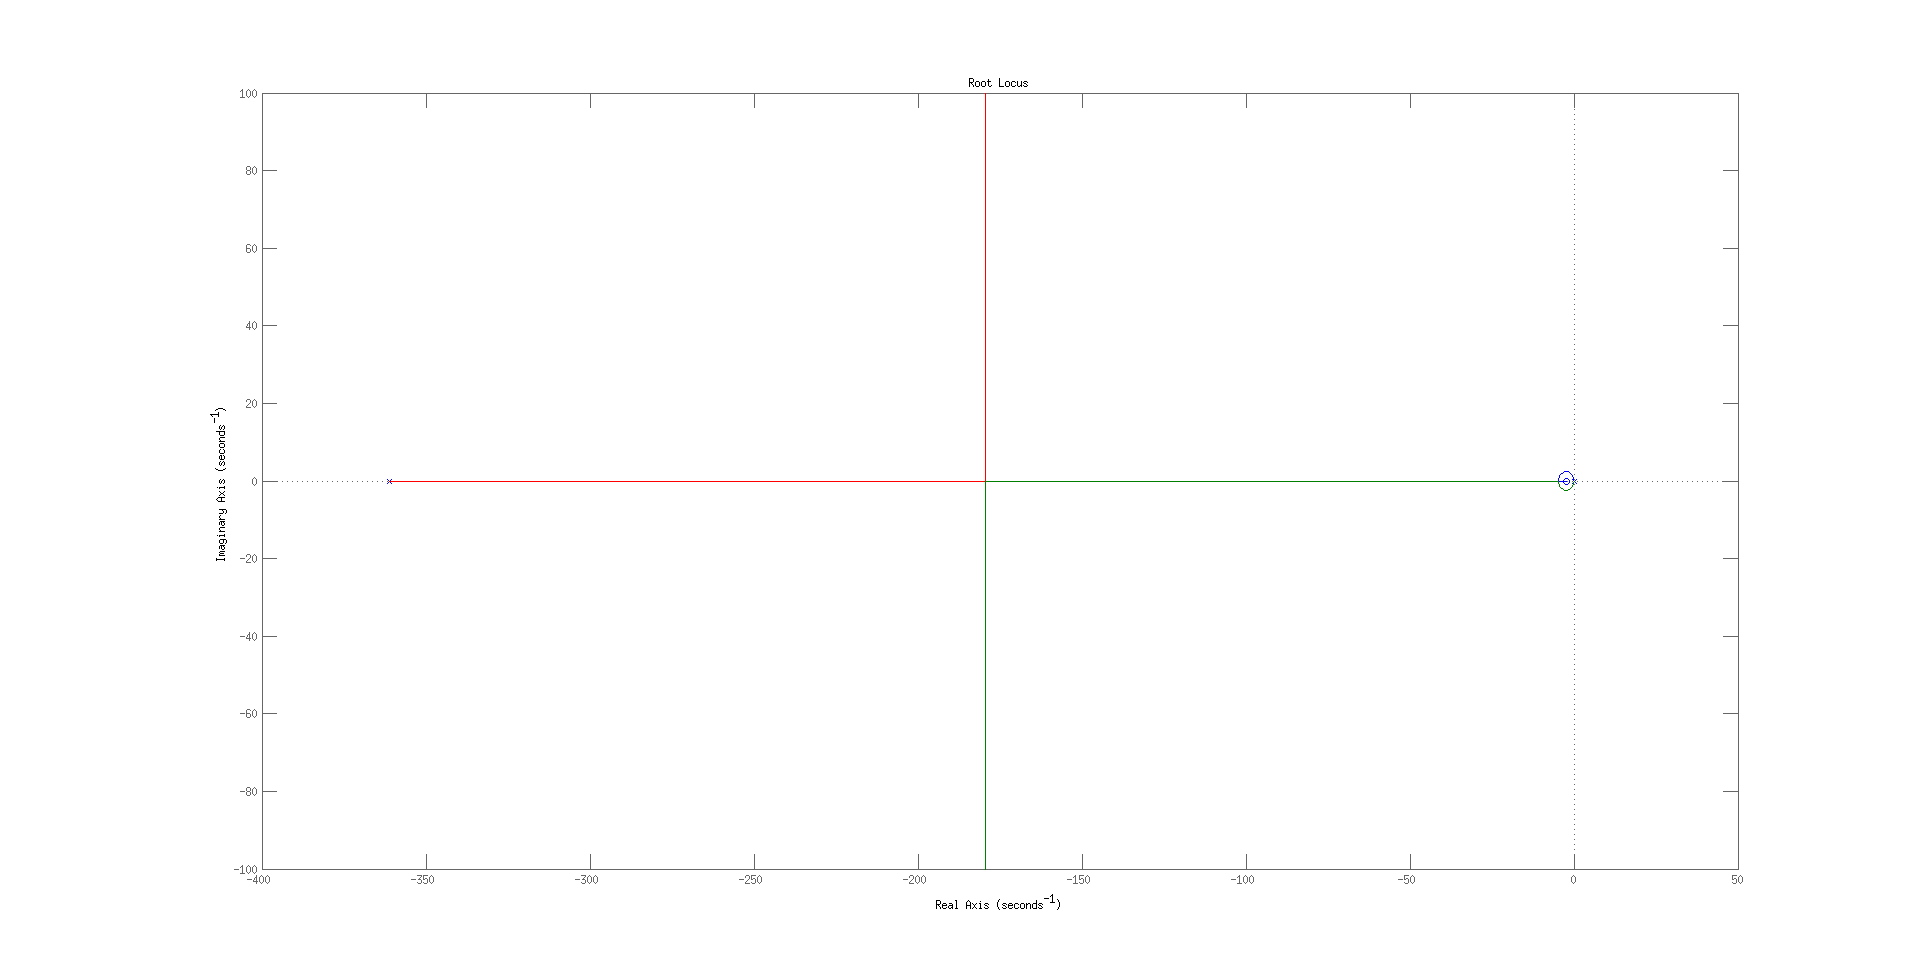
\includegraphics[width=\textwidth]{pi_rlocus.png}
 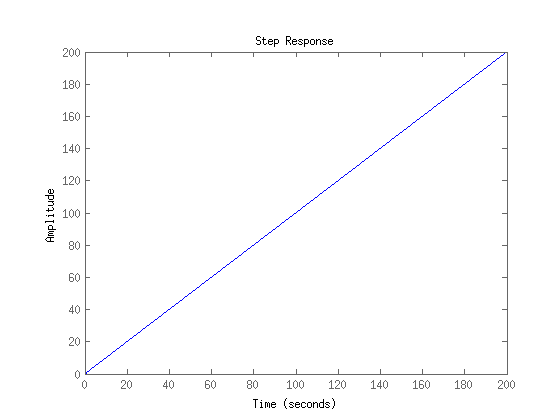
\includegraphics[width=\textwidth]{step2.png}

Επομένως $$G_c(s) = 11.7 + \frac {0.55} s$$

και η συνολική ΣΜΑΒ

$$G(s) = G_c(s) G_p(s) = \frac {4500(13 + 31.5 / s)}  {s (s + 361.2)}$$



\section*{3ο Ερώτημα} 

Στο παρόν ερώτημα θα χρησιμοποιήσουμε PID ελεγκτή με συνάρτηση μεταφοράς $$G_c(s) = k_p + \frac {k_i} s + s k_d$$ για τον έλεγχο της διάταξης $G_p(s)$. Η χαρακτηριστική εξίσωση για την εύρεση του γτρ (για $K = 1$) είναι η $$1 + G_c(s) G_p(s) = 0 \iff 2.718 \times 10^9 (s k_p + k_i + k_d s^2) + s^2 (s + 400.26) (s + 3008) = 0$$

\subsection*{Περιορισμοί Σχεδίασης \& Σχεδίαση PID Ελεγκτή} 

\paragraph{Περιορισμοί Σχεδίασης} 

Οι περιορισμοί σχεδίασης θέτουν προδιαγραφές για είσοδο $r(t) = t $ : $e_{ss} \le 0.000443, \; M_p \le 5 \%, \; T_r \le 0.005 \mathrm s, \; T_s \le 0.005 \mathrm s$.

Σχηματικά ο γτρ χωρίς τον ελεγκτή απεικονίζεται ως

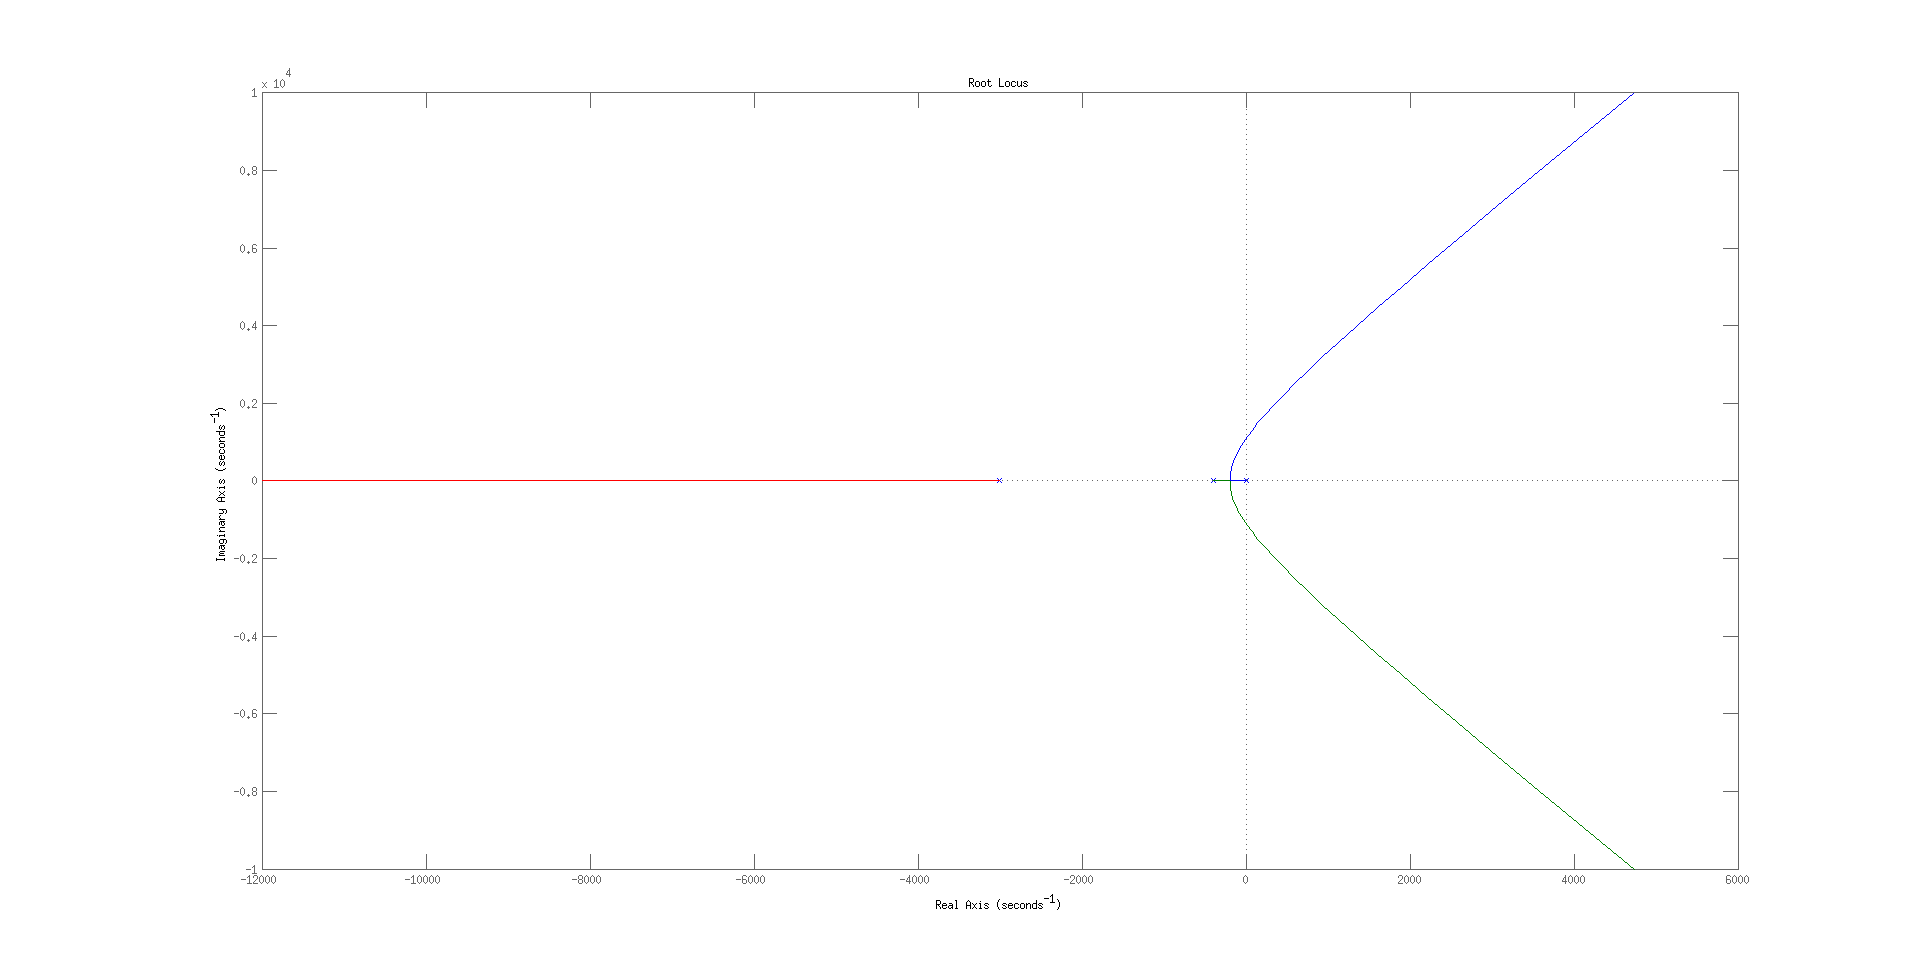
\includegraphics[width=\textwidth]{plant3_rlocus.png}
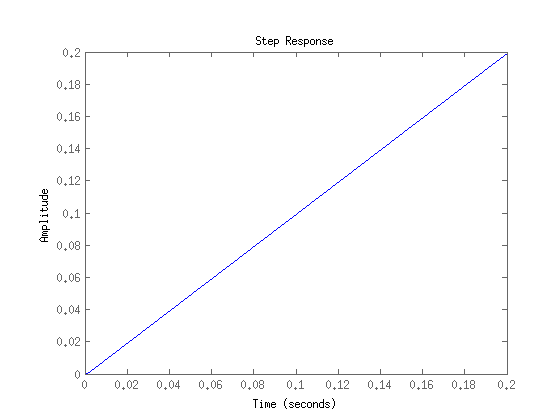
\includegraphics[width=\textwidth]{step3.png}


Το σύστημα είναι τύπου 1 και δεν χρειάζεται να αυξήσουμε τον τύπο του με ολοκληρωτή.  μπορούμε να θέσουμε $k_i = 0$ επομένως ανάγουμε την κατάσταση σε PD έλεγχο (Dorf) με $G_c(s) = k_p + k_d s = k_d (s + k_p / k_d) = k_d (s + z)$. Θέλουμε να πετύχουμε $M_p \le 5 \%, \; T_r \le 0.005 \; \mathrm{sec}, \; T_s \le 0.005 \; \mathrm {sec}$.
  
\paragraph{Επιλογή Κερδών Ελεγκτή} Χρησιμοποιώντας τον PID Tuner στο MATLAB καταλήγουμε ότι οι τιμές 

$$k_p = 0.37  \qquad k_d = 0.0008 \qquad k_i  = 0$$  

μας δίνουν ελεγκτή μέσα στις προδιαγραφές σχεδίασης και συγκεκριμένα

\begin{verbatim}
ans = 

        RiseTime: 0.0021
    SettlingTime: 0.0032
     SettlingMin: 0.9004
     SettlingMax: 1.0198
       Overshoot: 1.9839
      Undershoot: 0
            Peak: 1.0198
        PeakTime: 0.0050


Kv =

  835.2782


ess =

    0.0012

\end{verbatim}
  
Επομένως $$G_c(s) = 0.37 + 0.0008s$$  
  
  
Το σφάλμα ταχύτητας και το $e_{ss}$ είναι 

$$K_v = \lim_{s \to 0} s G_p(s) G_c(s) = 2.718 \times 10^9 \times k_p / 1203982.08, \qquad e_{ss} = 1 / K_v = 0.0012 \le 0.00443 $$  
  
Επομένως η συνολική ΣΜΑΒ είναι η 

$$G(s) = \frac {2.718 \times 10^9 (0.37 + 0.0008s)} {s(s + 400.26)(s + 3008)}$$  

και ο νέος γτρ της απεικονίζεται ακολούθως:

 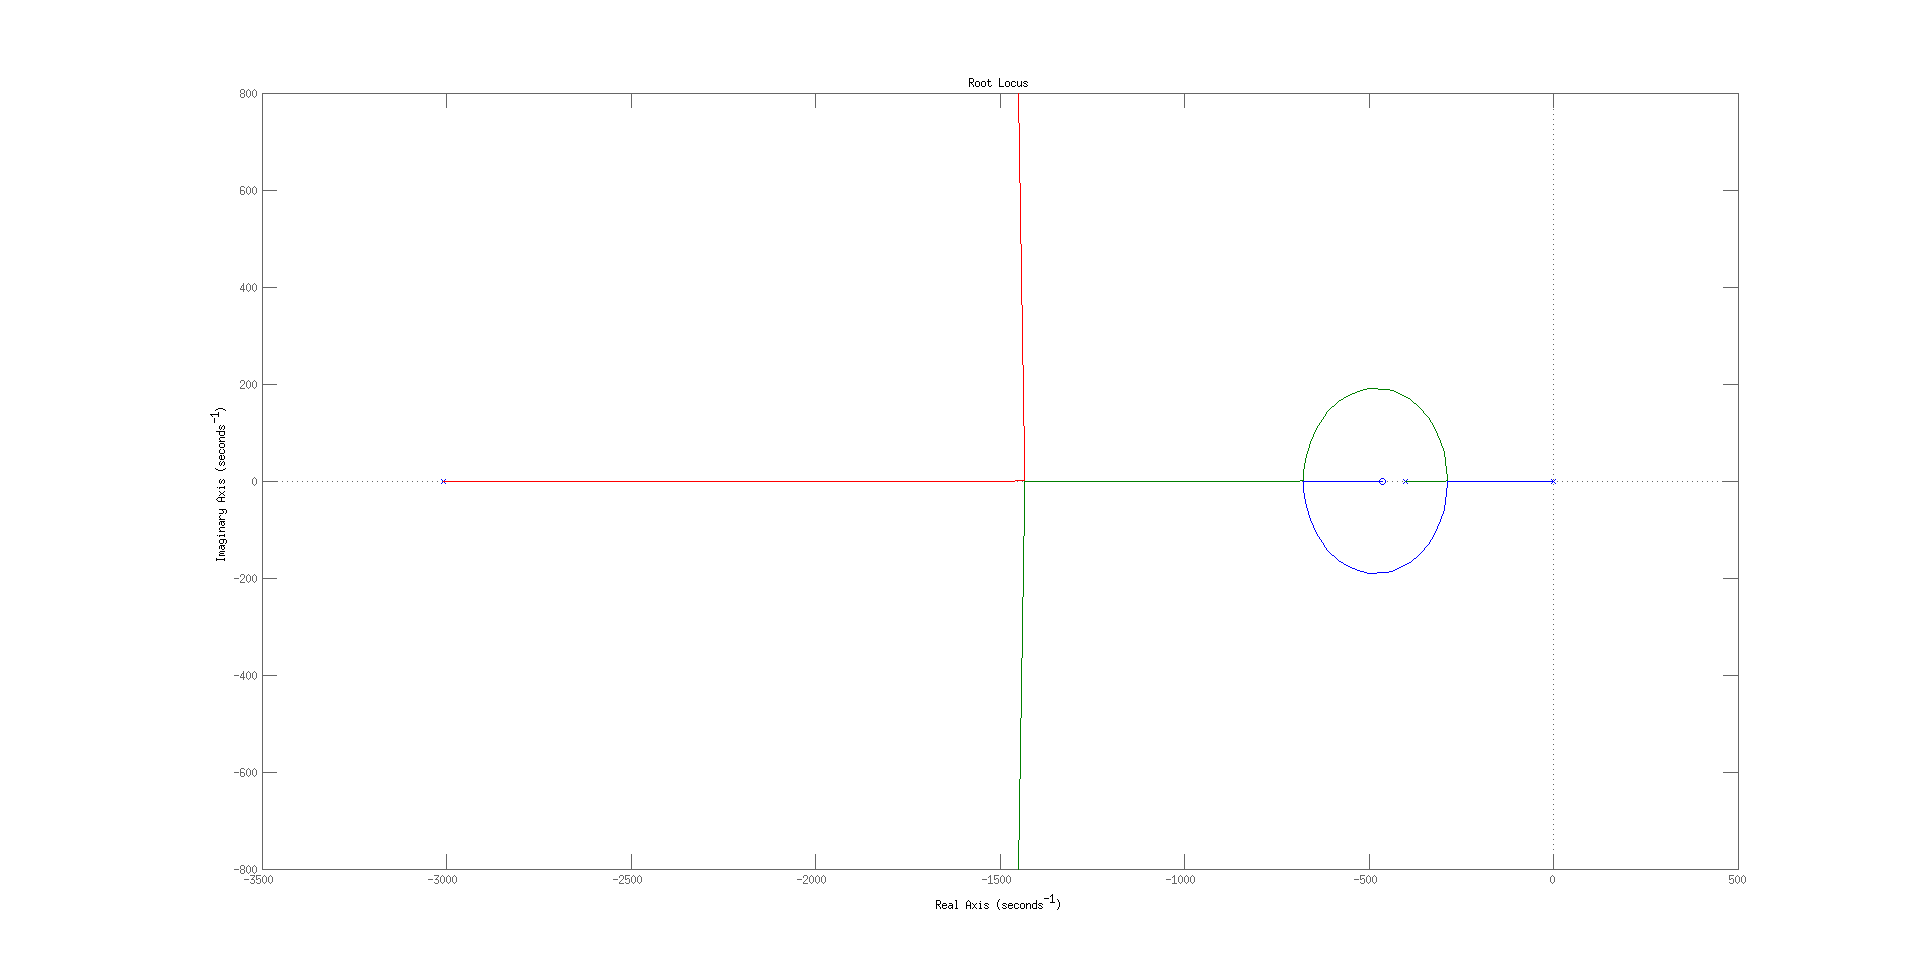
\includegraphics[width=\textwidth]{pd2_rlocus.png}




\section*{Αναφορές}

\noindent [1] Dorf, Richard C., and Robert H. Bishop. Modern control systems. Pearson, 2011.

\noindent [2] Paraskevopoulos, P. N. Modern control engineering. CRC Press, 2001.

\noindent [3] Ogata, Katsuhiko, and Yanjuan Yang. Modern control engineering. Vol. 4. India: Prentice hall, 2002.

\noindent [4] MATLAB/Simulink Reference Manual

\end{document}
